
\section{Packet Filtering}
\subsection{Purpose}
After whitelist has been extracted, we can keep the network traffic of IoT system secure by filtering unwanted traffic.  
The purpose of this experiment is to test our filtering method, 
\colorbox{white}{\lstinline[basicstyle=\ttfamily\color{black}]|iptables|}
 
\subsection{Method} 
 
In this experiment, we created a filter by combining 
\colorbox{white}{\lstinline[basicstyle=\ttfamily\color{black}]|NetfilterQueue-python|}
and \newline
\colorbox{white}{\lstinline[basicstyle=\ttfamily\color{black}]|iptables|}.
\colorbox{white}{\lstinline[basicstyle=\ttfamily\color{black}]|iptables|} is a Linux command that allows user to filter network packets by configure tables of IP packet filter rules in the Linux kernel. We wrote a program that take the JSON output of whitelist extraction program as an input a create an 
\colorbox{white}{\lstinline[basicstyle=\ttfamily\color{black}]|iptables|}
iptables script as its output. Next is the template of our script.
\\

\lstset{
  breaklines = true,
  classoffset=1,
  frame=tRBl,
  framesep=5pt,
  showstringspaces=false,
  numbers=left,
  stepnumber=1,
  tabsize=2,
}


\begin{lstlisting}[label=sh]
# iptables -F  
# iptables -P ACCEPT
# iptables -A FORWARD -p [udp|tcp] -dport [port number] -d [Host IP] -s [Device IP] -j ACCEPT 
# iptables -A FORWARD -p [udp|tcp] -dport [port number] -d [Device IP] -s [Host IP] -j ACCEPT
# iptables -A FORWARD -p [udp|tcp] -j DROP 
\end{lstlisting}

\begin{itemize}
    \item 1st line, -F command is to clean the exist rule in iptables. 
    \item 2nd line states that our default policy to ACCEPT. In other words, packet that doesn't match with any rule in iptables will be forwarded.
    \item 3rd and 4th line states that only device’s hosts with specific protocol, port number can communicate with the device.
    \item 5th line means any tcp,udp packet that doesn't match above rules will be dropped.
\end{itemize}

Then we ran this script on computer bridging between the internet and the switch. This allowed us to filter all unnecessary packets and kept our IoT system secure. 
Next step, we wanted to evaluate the performance of our whitelist. 
Therefore, instead of dropping and accepting at the iptables, we configured iptables to pass all dropped packets to our “NetfilterQueue” python program. NetfilterQueue is a module that provides access to packets matched by iptables rule, we can analyze those packets using “kamene” (also known as “scapy”).
(Figure \ref{fig:s4_netfilter})

\begin{figure}[h]
    \centering 
    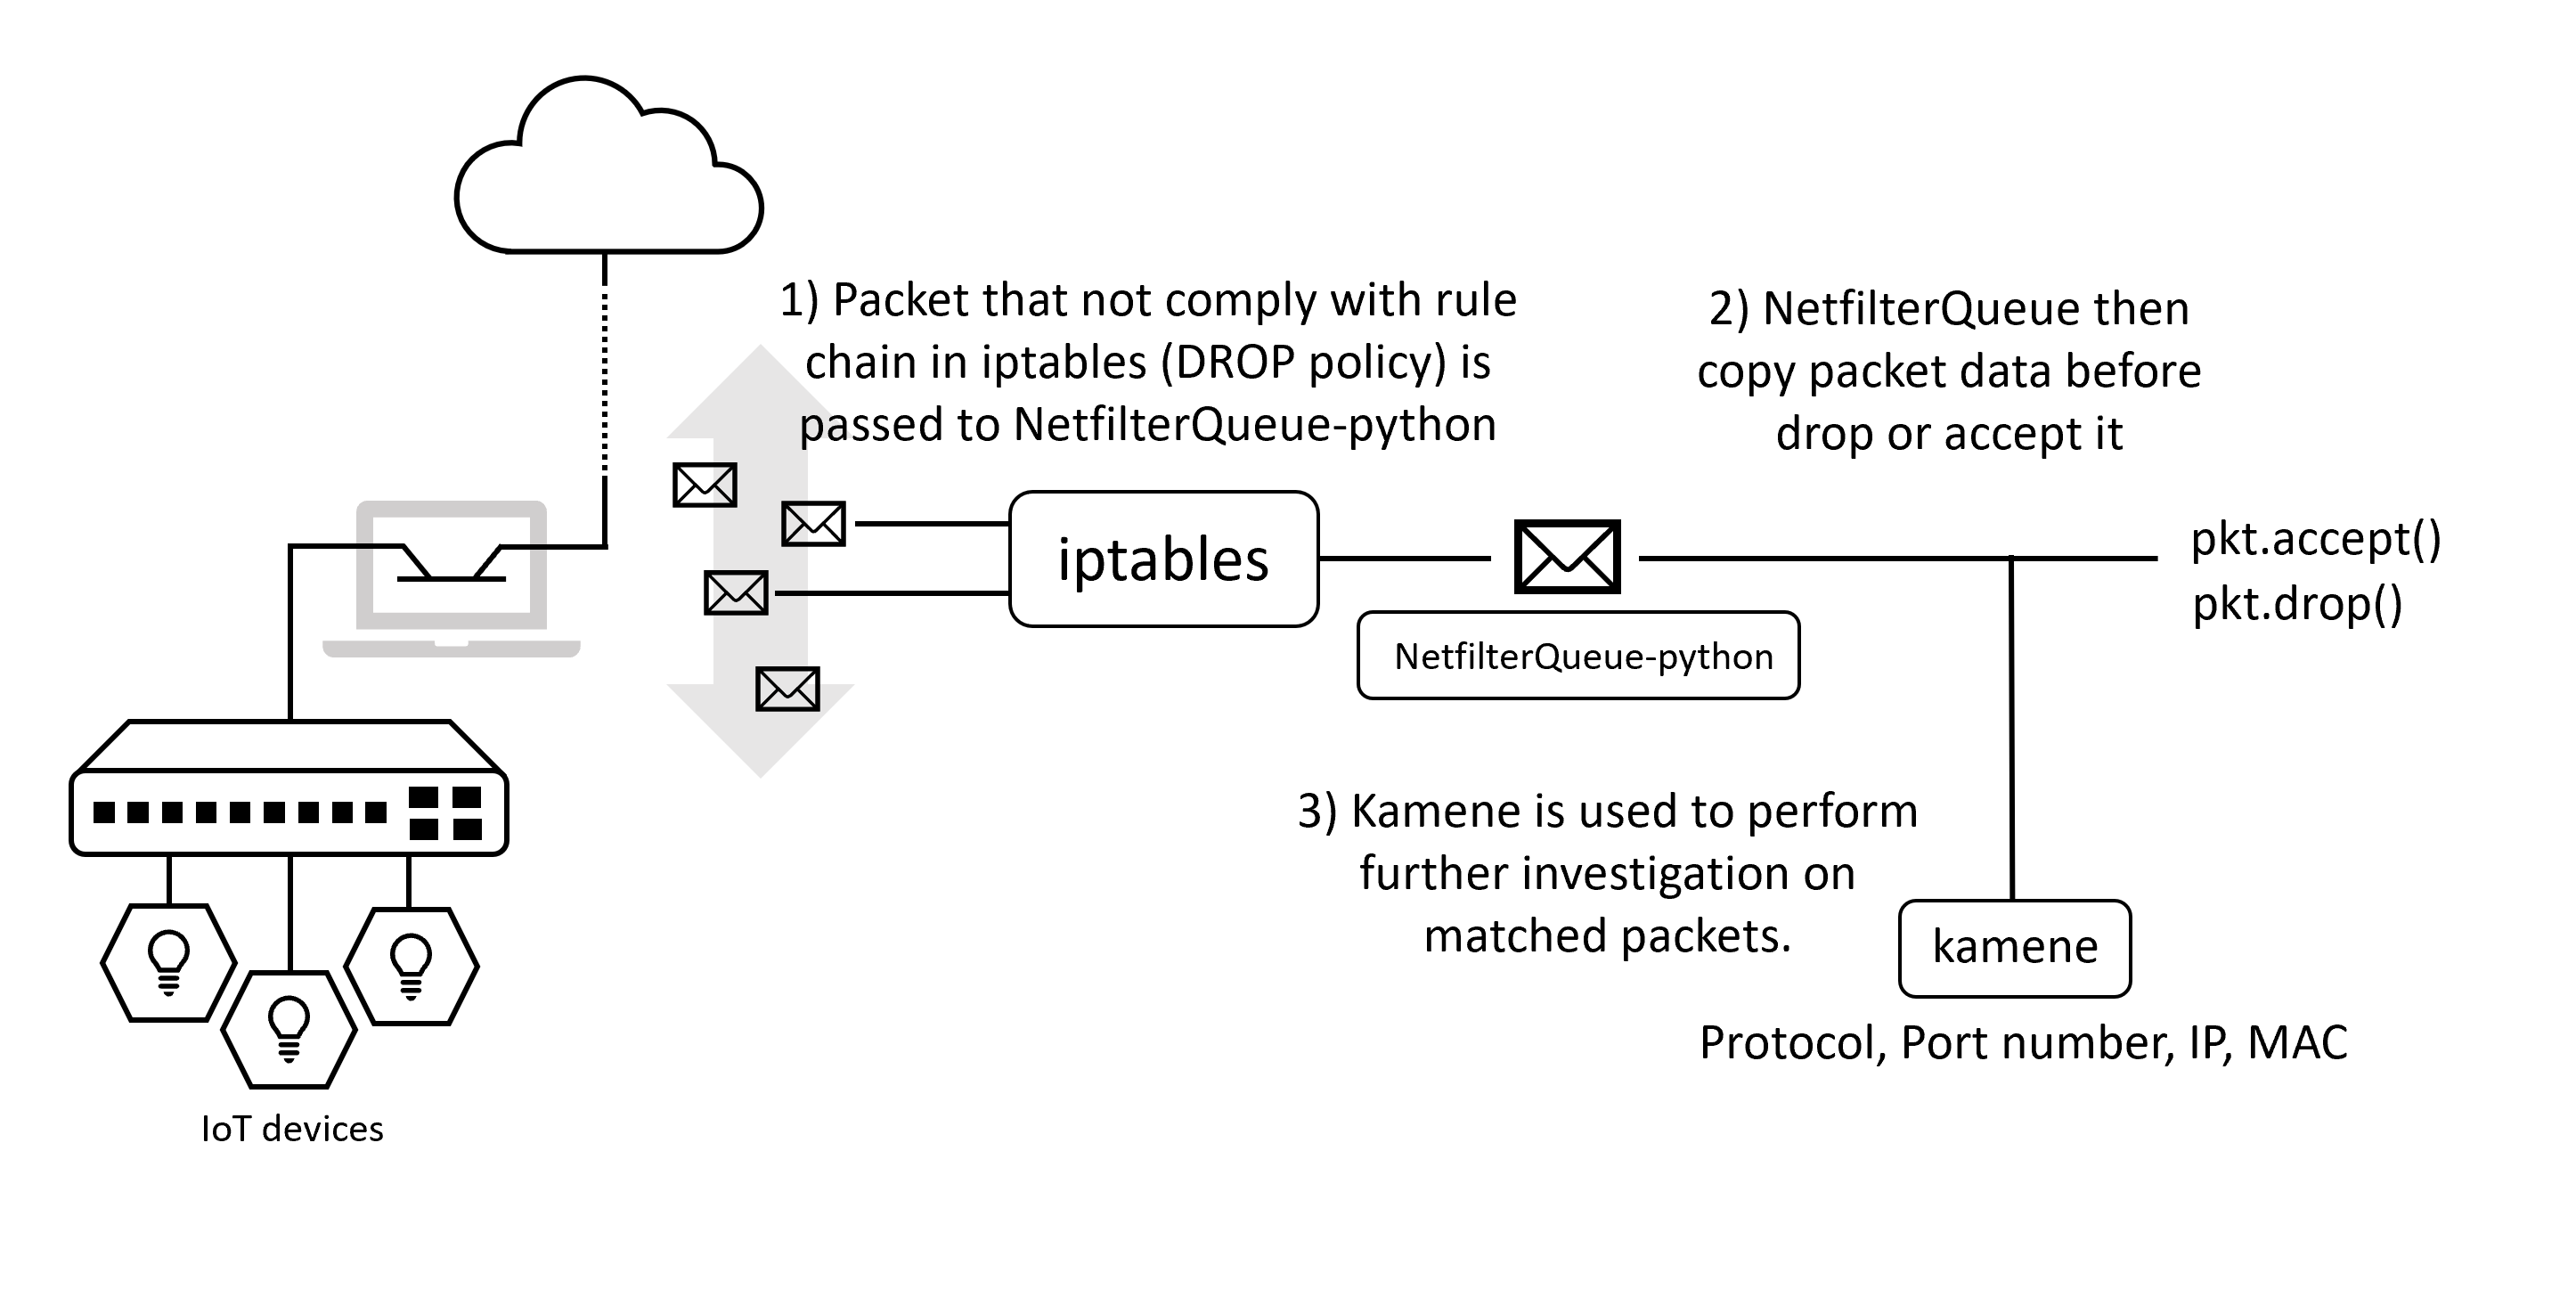
\includegraphics[width=\textwidth]{4_netfilter} 
    \caption{Analyzing matched packet using NetfilterQueue-python module and kamene}
    \label{fig:s4_netfilter}
\end{figure} 

We had filtered the network traffic of eroom from 24 January 2019 to 30 January 2019. 
During this period no intentional attack was conducted.

\subsection{result}
We summarize all packet data that was sent to NetfilterQueue.
The dropped packet is divided into 3 category: 
\begin{itemize}
    \item Host-dropped packet : A packet which is destinated for devices but doesn't comply with the rule.
    \item Device-dropped packet : A packet which is originated from our devices but doesn't comply with our iptables rule.
    \item Unrelated packet : A packet which source or destination IP isn't marked for our IoT devices.
\end{itemize}
As a primary evaluation method, we believe that the system should has low Device-dropped packet number
while all the Host-dropped packet should be from unknown source.

\newpage 

\subsubsection{Host-dropped packet}  
 
\begin{table}[h]
    \caption{Host-dropped packet }
    \label{table:s4_host_drop}
    \centering
    \begin{tabular*}{\textwidth}{ @{\extracolsep{\fill}} lll}
        \toprule
        \textbf{Protocol}             & \textbf{Source}          & \textbf{Host Location} \\  \toprule 
        \multirow{4}{*}{TCP/22}     & 75.151.236.50     & USA           \\ 
                                    & 78.128.112.62     & Bulgaria      \\
                                    & 114.156.2.98      & Japan (JPNIC) \\
                                    & 185.209.0.12      & Latvia (VPN)  \\ \cline{1-3}
        tcp/1886                    & 185.222.211.146   & UK            \\ \cline{1-3}
        \multirow{4}{*}{TCP/1888}   & 85.93.20.22       & Bulgaria      \\
                                    & 114.156.2.98      & Japan (JPNIC) \\
                                    & 198.108.67.32     & USA           \\
                                    & 198.108.67.48     & USA           \\ \bottomrule
    \end{tabular*} 
\end{table}

Table \ref{table:s4_host_drop} summarizes, packets from host which is not in device's whitelist. 
All the packet is destined for EchoNetLiteGW (192.168.10.10). 
TCP/22 is the SSH port (Secure Shell), adversaries normally guess the password and try logging in to the device through this port. If the 22 port is opened and device’s configuration allow logging in by password, there is a chance that our devices might get hacked.

\subsubsection{Device-dropped}
\begin{table}[h]
    \caption{Device-dropped packet }
    \label{table:s4_device_drop}
    \centering
    \begin{tabular*}{0.6\textwidth}{ @{\extracolsep{\fill}} lll}
        \toprule
        \textbf{Protocol}           & \textbf{Source}   & \textbf{Destination} \\  \toprule 
        \multirow{3}{*}{TCP/3610}   & 192.168.10.11     &  \multirow{3}{*}{224.0.23.0} \\           
                                    & 192.168.10.12     &  \\
                                    & 192.168.10.13     &  \\
        \bottomrule
    \end{tabular*} 
\end{table}
The device-dropped packets are TCP/3610 packets originated from Control panel (.11) and two air conditioners (.12 .13) destined for 224.0.23.0.  

In EchoNetLite protocol, 224.0.13.0 is the broadcast IP address, so we believe that this IP should be added to the whitelist. After we investigated traffic data, we found that IoT devices used broadcast less than 10 times during filtered period. We assumed that reason it wasn’t added to the whitelist is because, our dataset was too short and that it didn’t contain broadcast packet.  

\subsubsection{Unrelated packet}  
We had UDP/67 source 0.0.0.0, destination 255.255.255.255 as our unrelated packet. This packet pattern can be found in dynamic host configuration protocol. However, our IoT devices have their allocated IP address, therefore there was no necessary for using DHCP.
\\ \\
From this result, we knew the our system was working, and we have protected our device from potential attack.
 